\begin{apendicesenv}

\partapendices



\chapter{Estudo de viabilidade} \label{appendix:estudo_viabilidade}

\par A pesquisa foi dividida em dois formulários, sendo um exclusivo para cadeirantes e o outro para os representantes de supermercado. O primeiro formulário tem como objetivos:

\begin{itemize}  
\item Buscar as características do público alvo do projeto;
\item Identificar o volume das compras realizado por cadeirantes;
\item Identificar a dificuldade em realizar compras por parte dos cadeirantes;
\item Verificar a aceitação e o interesse do público alvo pelo projeto a ser implementado;
\item Levantar sugestões de aprimoramento do produto de acordo com a visão do público alvo;
\end{itemize}

\par O segundo formulário tem como objetivos:

\begin{itemize}  
\item Buscar as características do público alvo do projeto de acordo com a visão dos representantes de supermercado;
\item Identificar ferramentas de suporte aos cadeirantes já oferecidas pelos supermercados;
\item Verificar a aceitação e o interesse por parte dos supermercados em implementar o produto;
\item Identificar uma margem de custo na qual o supermercado estaria disposto a pagar pelo produto;
\end{itemize}

\par Para validar o objetivo do estudo o questionário foi implementado na plataforma \textit{Typeform}. Essa plataforma permite que os usuários respondam o questionário de forma virtual, tanto em computadores quanto com \textit{smartphones}, otimizando o processo da pesquisa. Foram feitas 18 perguntas, sendo 12 perguntas para o questionário voltado para os cadeirantes e 6 perguntas voltadas para os representantes  de supermercados. O resultado é apresentado na Tabela \ref{tab:quest_viabilidade}.

\begin{sidewaystable}[]
\centering
\caption{Resultado do questionário do estudo de viabilidade.}
\label{tab:quest_viabilidade}
\resizebox{\textwidth}{!}{%
\begin{tabular}{lll}
Pergunta                                                                               & Propósito                                                                                    & Resultados                                      \\
Sexo                                                                                   & Identificar o perfil dos respondentes                                                        & Masculino                                       \\
Idade                                                                                  & Identificar o perfil dos respondentes                                                        & 45 a 60 anos                                    \\
Qual o modelo da cadeira de rodas?                                                     & Buscar características do público alvo                                                       & Automatizada                                    \\
Possui veículo próprio?                                                                & Buscar características do público alvo                                                       & Não                                             \\
Faz compras no supermercado?                                                           & Buscar características e identificar o perfil do público alvo                                & Sim                                             \\
Realiza compras acompanhado(a)?                                                        & Buscar características e identificar o perfil do público alvo                                & Sempre/ ás vezes                                \\
Quanta vez no mês frequenta o supermercado?                                            & Buscar características e identificar o perfil do público alvo                                & Mais de 4 vezes                                 \\
Qual o volume de compras por cada ida ao supermercado?                                 & Identificar o volume das compras realizado por cadeirantes                                   & Médio                                           \\
Caso vá sozinho, o supermercado oferece algum serviço para auxiliá-lo?                 & Identificar a dificuldade em realizar compras por parte dos cadeirantes                      & Não                                             \\
Quais as principais dificuldades que encontra no supermercado?                         & Identificar a dificuldade em realizar compras por parte dos cadeirantes                      & Carregar as compras / Pegar itens na prateleira \\
Um carrinho autônomo você acha que pode auxiliar nesse processo?                       & Verificar a aceitação e o interesse do público alvo pelo projeto a ser implementado          & Sim                                             \\
Quais aspectos o carrinho autônomo deve oferecer?                                      & Levantar sugestões de aprimoramento do produto de acordo com a visão do público alvo         & Altura,Volume e Velocidade                      \\
Á frequente a presença de clientes cadeirantes no supermercado?                        & Buscar características e identificar o perfil do público alvo                                & Não / Sim (50\% pra cada)                       \\
Quais serviços de auxilio o supermercado oferece?                                      & Identificar ferramentas de suporte aos cadeirantes já oferecidas pelos supermercados         & Acessibilidade                                  \\
Seria interessante implementar carrinhos autônomos para auxiliar os cadeirantes?       & Verificar a aceitação e o interesse por parte dos supermercados em implementar o produto     & Sim                                             \\
O quanto o supermercado estaria disposto a pagar pelo produto?                         & Identificar uma margem de custo na qual o supermercado estaria disposto a pagar pelo produto & R\$ 500 a R\$ 1000                                \\
O supermercado acredita que o carrinho autônomo pode oferecer diferencial competitivo? & Verificar a aceitação e o interesse por parte dos supermercados em implementar o produto     & Sim                                             \\
Os cadeirantes que frequentam o supermercado vão sozinhos ou acompanhados por alguém?  & Buscar características e identificar o perfil do público alvo                                & Sozinhos                                       
\end{tabular}}
\end{sidewaystable}


\chapter{Planos de gerenciamento} \label{appendix:planos}

\section{Plano de gerenciamento de escopo}

O processo de gerenciamento de escopo conforme propõe o PMBOK envolve os seguintes processos:

\begin{itemize}
\item Coletar os requisitos;
\item Definir o escopo;
\item Criar a EAP;
\item Validar o escopo;
\item Controlar o escopo.
\end{itemize}

No contexto do presente projeto, o gerenciamento do escopo se dará conforme explicitado na Figura \ref{fig:escopo}. Será necessário o envolvimento de toda a equipe desde a concepção do projeto ao seu término. Os professores que orientam este trabalho serão responsáveis por auxiliar nesse processo validando as ideias em termos técnicos e sugerindo alternativas. Caberá aos gerentes do projeto e aos subgerentes a responsabilidade de monitorar a equipe do projeto para garantir que o processo de controle de escopo (Figura \ref{fig:escopo}) seja executado conforme o previsto. Todas solicitações de mudanças devem passar primeiramente pelos subgerentes e posteriormente a toda a equipe. Para uma mudança ser aprovada deve ser realizada tanto a aprovação pela equipe quanto pelos professores orientadores.

\begin{figure}[htpb!]
    \centering
    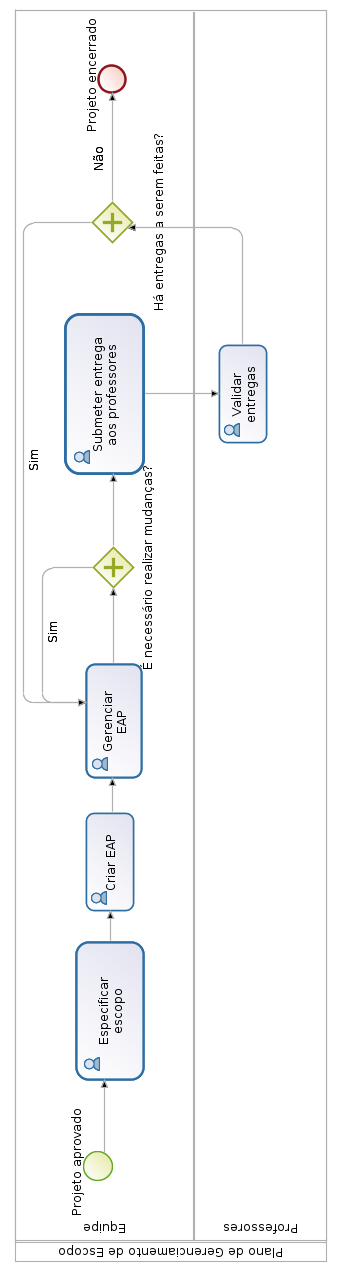
\includegraphics[scale= 0.7]{figuras/escopo.png}
    \caption[Escopo]{Plano de Gerenciamento de Escopo. Fonte: Autores.}
    \label{fig:escopo}
\end{figure}

\subsection{Objetivos}

Tratando-se de um projeto que relaciona diferentes engenharias e tanto aspectos teóricos quanto práticos, será necessário atender aos seguintes objetivos:

\begin{itemize}
\item Monitorar o status do escopo do projeto;
\item Rastrear mudanças;
\item Controlar impactos das mudanças no escopo geral.
\end{itemize}

Deste modo, será possível entregar o produto conforme planejado.

\subsection{Artefatos que definem o escopo}
Os artefatos que fazem parte do gerenciamento do escopo e que o definem são:

\begin{itemize}
\item Declaração do escopo %\ref{};
\item Estrutura Analítica do Projeto (Figura \ref{fig:eap_projeto});
\item Estrutura Analítica do Produto (Figura \ref{fig:eap_produto}).
\end{itemize}

\subsection{Estrutura Analítica do Projeto e do Produto}

Para comunicar os entregáveis que compõem o produto, foi ilustrada a EAP do produto conforme a Figura \ref{fig:eap_produto}.

\begin{figure}[htpb!]
    \centering
    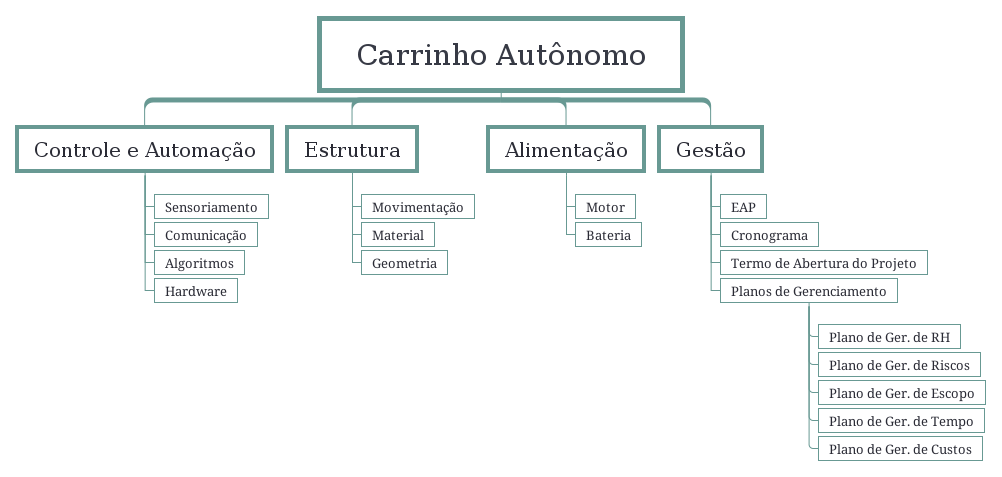
\includegraphics[scale= 0.5]{figuras/eap_produto.png}
    \caption{EAP do Produto. Fonte: Autores.}
    \label{fig:eap_produto}
\end{figure}

Para comunicar os entregáveis que compõem o projeto, foi ilustrada a EAP do projeto conforme a Figura \ref{fig:eap_projeto}.

\begin{figure}[htpb!]
    \centering
    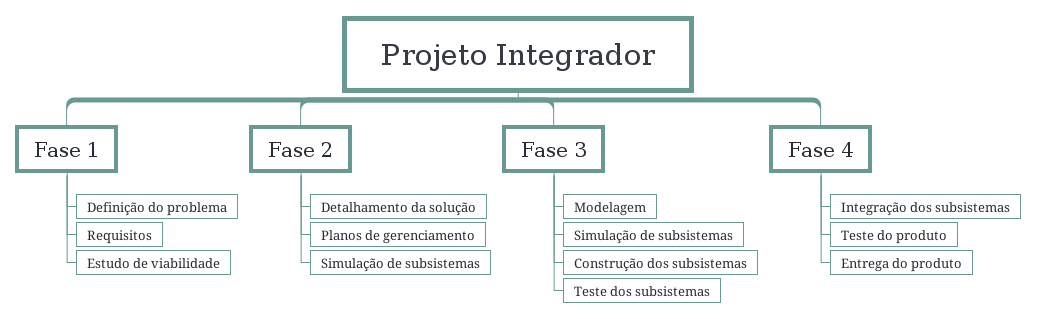
\includegraphics[scale= 0.5]{figuras/eap_projeto.png}
    \caption{EAP do Projeto. Fonte: Autores.}
    \label{fig:eap_projeto}
\end{figure}

\newpage

\section{Plano de gerenciamento de recursos humanos}

O processo de gerenciamento de recursos humanos conforme propõe o PMBOK envolve os seguintes processos:

\begin{itemize}
\item Mobilizar a equipe do projeto;
\item Desenvolver a equipe do projeto;
\item Gerenciar a equipe do projeto.
\end{itemize}

No contexto do presente projeto, o gerenciamento do escopo se dará conforme explicitado na Figura \ref{fig:rh}. 

\begin{figure}[htpb!]
    \centering
    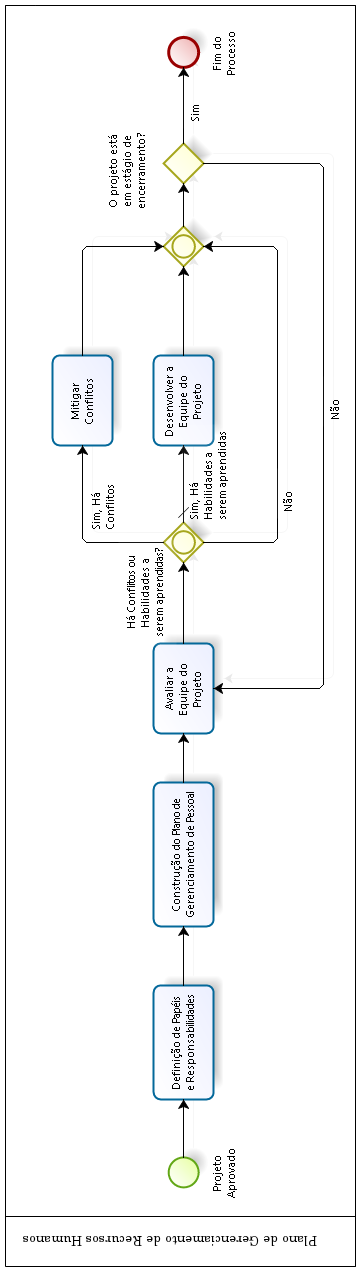
\includegraphics[scale= 0.7]{figuras/rh.png}
    \caption[RH]{Plano de Gerenciamento de RH. Fonte: Autores.}
    \label{fig:rh}
\end{figure}

\newpage

\subsection{Responsabilidades}
Os recursos humanos que foram mobilizados para este projeto e suas responsabilidades são detalhados na Tabela \ref{tab:responsabilidades}.


% ######## init table ########
\begin{table}[h]
\caption {Detalhamento das responsabilidades} \label{tab:responsabilidades} 
 \centering
% distancia entre a linha e o texto
 {\renewcommand\arraystretch{1.25}
 \begin{tabular}{ l l l }
  \cline{1-1}\cline{2-2}\cline{3-3}  
    \multicolumn{1}{|p{2.567cm}|}{Papel} &
    \multicolumn{1}{p{6.433cm}|}{Responsabilidade} &
    \multicolumn{1}{p{2.417cm}|}{Responsáveis}
  \\  
  \cline{1-1}\cline{2-2}\cline{3-3}  
    \multicolumn{1}{|p{2.567cm}|}{Equipe} &
    \multicolumn{1}{p{6.433cm}|}{Planejar e desenvolver o carrinho considerando aspectos de engenharia.} &
    \multicolumn{1}{p{2.417cm}|}{Todos}
  \\  
  \cline{1-1}\cline{2-2}\cline{3-3}  
    \multicolumn{1}{|p{2.567cm}|}{Engenheiro Aeroespacial} &
    \multicolumn{1}{p{6.433cm}|}{Definir e desenvolver a estrutura do carrinho.} &
    \multicolumn{1}{p{2.417cm}|}{Allan}
  \\  
  \cline{1-1}\cline{2-2}\cline{3-3}  
    \multicolumn{1}{|p{2.567cm}|}{Engenheiro Automotivo} &
    \multicolumn{1}{p{6.433cm}|}{Definir e promover a movimentação do carrinho.} &
    \multicolumn{1}{p{2.417cm}|}{Tharcísio e Thayza}
  \\  
  \cline{1-1}\cline{2-2}\cline{3-3}  
    \multicolumn{1}{|p{2.567cm}|}{Engenheiro de Energia} &
    \multicolumn{1}{p{6.433cm}|}{Definir e promover a alimentação do carrinho.} &
    \multicolumn{1}{p{2.417cm}|}{Caio, Lorrane, Lucas e Taís}
  \\  
  \cline{1-1}\cline{2-2}\cline{3-3}  
    \multicolumn{1}{|p{2.567cm}|}{Engenheiro Eletrônico} &
    \multicolumn{1}{p{6.433cm}|}{Definir, desenvolver e configurar equipamentos eletrônicos.} &
    \multicolumn{1}{p{2.417cm}|}{Isabela, Paulo e Yan}
  \\  
  \cline{1-1}\cline{2-2}\cline{3-3}  
    \multicolumn{1}{|p{2.567cm}|}{Engenheiro de Software} &
    \multicolumn{1}{p{6.433cm}|}{Desenvolver algoritmos de controle do carrinho.} &
    \multicolumn{1}{p{2.417cm}|}{Dandara, Danilo e Tainara}
  \\  
  \cline{1-1}\cline{2-2}\cline{3-3}  
    \multicolumn{1}{|p{2.567cm}|}{Gerente do projeto} &
    \multicolumn{1}{p{6.433cm}|}{Acompanhar escopo do projeto.  			

Ter iniciativa para a tomada de decisões.  			

Organizar pauta das reuniões } &
    \multicolumn{1}{p{2.417cm}|}{Dandara, Isabela e Tainara}
  \\  
  \cline{1-1}\cline{2-2}\cline{3-3}  
    \multicolumn{1}{|p{2.567cm}|}{Subgerentes do projeto} &
    \multicolumn{1}{p{6.433cm}|}{Comunicar andamento das atividades planejadas.} &
    \multicolumn{1}{p{2.417cm}|}{Lucas, Paulo e Tharcísio}
  \\  
  \cline{1-1}\cline{2-2}\cline{3-3}  
    \multicolumn{1}{|p{2.567cm}|}{Subgrupo - Alimentação} &
    \multicolumn{1}{p{6.433cm}|}{Trabalho conjunto para garantir a alimentação do carrinho.} &
    \multicolumn{1}{p{2.417cm}|}{Caio, Lorrane, Lucas e Taís}
  \\  
  \cline{1-1}\cline{2-2}\cline{3-3}  
    \multicolumn{1}{|p{2.567cm}|}{Subgrupo - Controle} &
    \multicolumn{1}{p{6.433cm}|}{Trabalho conjunto entre alunos de Engenharia de Software e Engenharia Eletrônica para garantir o controle da movimentação do carrinho. } &
    \multicolumn{1}{p{2.417cm}|}{Paulo, Danilo, Dandara, Isabela, Tainara e Yan}
  \\  
  \cline{1-1}\cline{2-2}\cline{3-3}  
    \multicolumn{1}{|p{2.567cm}|}{Subgrupo - Estrutura} &
    \multicolumn{1}{p{6.433cm}|}{Trabalho conjunto entre alunos de Engenharia Automotiva e Aeroespacial para garantir a estrutura adequada do carrinho.} &
    \multicolumn{1}{p{2.417cm}|}{Allan, Tharcísio e Thayza}
  \\  
  \hline

 \end{tabular} }
\end{table}

\newpage

\subsection{Gerenciamento das reuniões}

A equipe possui dois encontros presenciais obrigatórios:

\begin{itemize}
  \item Às quartas-feiras: com duração de duas horas, a reunião inicia com \textit{stand-up meeting} de 5 minutos entre as gerentes e os subgerentes do projeto para que forneçam \textit{feedbacks}. Em seguida os subgrupos se reunem por uma hora e posteriormente há reunião geral para discutir a pauta;
  \item Às sextas-feiras: com duração de quatro horas, a reunião também se inicia com \textit{stand-up meeting}, porém, com a participação de todos, e segue conforme a necessidade ou a pauta.
\end{itemize}

\subsection{Desenvolvimento de habilidades}

Os subgerentes estão encarregados de acompanhar o desempenho dos membros da equipe fornecendo \textit{feedbacks} constantes às gerentes do projeto para levantar a necessidade de treinamentos para capacitar a equipe em algum quesito técnico necessário. Professores serão consultados durante todo o projeto para auxiliar nestes quesitos.




\section{Plano de gerenciamento de tempo}

O cronograma é uma forte ferramenta de organização temporal das atividades de um projeto,assim se faz necessário definir procedimentos para o controle do mesmo, a fim de manter o desenvolvimento do projeto sob controle e mantê-lo dentro do prazo estimado. Sendo assim o objetivo deste plano é estabelecer as diretrizes, que a equipe adotou, para realizar o controle do cronograma.


\subsection{Processos de Gerenciamento do tempo}
Segundo o PMBOK, existem 7 processos para o gerenciamento do tempo. E estes são os processos adotados pelo grupo:

\textbf{1. Planejar o gerenciamento do cronograma}

\textbf{2. Definir as atividades}

\textbf{3. Sequenciar as atividades}

\textbf{4. Estimar recursos das atividades}

\textbf{5. Estimar duração das atividades}

\textbf{6. Desenvolver o cronograma}

\textbf{7. Controlar o cronograma}

\subsection{Atividades}

A definição das atividades do projeto foram feitas levando em consideração a Estrutura Analítica do Projeto, os grandes marcos do projeto e os requisitos solicitados pelo professor. As atividades foram divididas para que fosse possível a execução destas em um espaço de tempo aceitável. 

\subsection{Cronograma}

Para uma melhor organização do projeto foi desenvolvido um cronograma geral utilizando a ferramenta do google chamada Gantter. A partir dele cada subgrupo criou seu próprio cronograma com atividades mais detalhadas. Na figura (Figura \ref{fig:cronogramaGeral}) pode-se visualizar o cronograma geral do projeto.

\begin{figure}[htpb!]
    \centering
    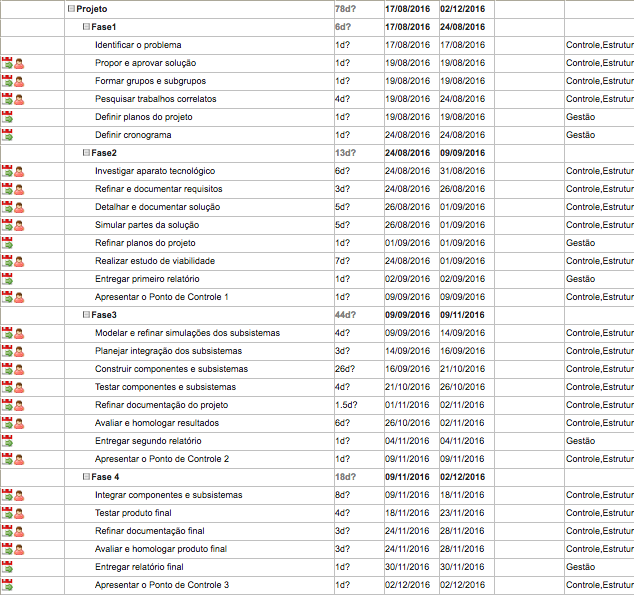
\includegraphics[scale= 0.7]{figuras/CronogramaGeral.png}
    \caption[Escopo]{Plano de Cronograma Geral do Projeto. Fonte: Autores.}
    \label{fig:cronogramaGeral}
\end{figure}

\subsubsection{Designando responsáveis para atividades}
O desenvolvimento de cada tarefa do cronograma é designada a pelo menos um dos integrantes do grupo. Os responsáveis foram escolhidos de acordo com a sua afinidade com a atividade e disponibilidade, e eles são também responsáveis por atualizar o status de suas atividades no cronograma do projeto.

\subsection{Responsáveis pela manutenção do cronograma}
O cronograma foi desenvolvido pelos integrantes do projeto contendo as principais atividades, as datas de entrega e o tempo estimado para se desenvolver cada atividade. Uma equipe de gestão foi definida, e essa equipe é responsável em manter datas, responsáveis e tempo estimado de cada atividade. 

\subsection{Controle de mudanças}
Todas as possíveis mudanças no projeto serão analisadas pelo grupo, pois uma mudança pode afetar o escopo, tempo e custo do projeto. O time irá reagir a esta mudança decidindo se esta irá ser desenvolvida ou não seguindo os planos de gerenciamento de escopo e riscos do projeto. Caso a mudança seja aceita isto refletirá no cronograma e a equipe de gestão será responsável em acomodar a mudança. Caso a mudança seja inevitável, a equipe deve moldar as atividades do cronograma para minimizar ao máximo os impactos negativos de tal mudança.


\section{Plano de gerenciamento de custos}

O principal objetivo deste plano é documentar a estimativa, planejamento e gerenciamento dos custos de todo o projeto.

\subsection{Estimar custos: recursos humanos do projeto} \label{subsec:custos_rh}

O projeto será desenvolvido por treze alunos da disciplina "Projeto Integrador 2" dos cursos de graduação da Universidade de Brasília - Faculdade UnB Gama. Baseado no Relatório de Gestão 2015 da Universidade de Brasília \cite{unb2015}, um aluno custou R\textdollar{ 16.640,00} no ano de 2015 Considerando que um ano letivo tem 200 dias, podemos calcular um custo de aluno como sendo de R\textdollar{ 83,20} por dia. Considere que a média de créditos que um aluno cursa por semestre como(máximo de créditos + mínimo de créditos)/2 = 24. 

Com esse valor podemos deduzir que o média de quantidade de horas por dia de um aluno é 5h. Sendo assim podemos deduzir que o preço do aluno por hora é de R\textdollar{  16,64}.
Levando esses dados em conta e considerando que um aluno trabalhe 8h por semana no projeto, o aluno custará: R\textdollar{ 133,12} por semana.
Considerando que o projeto tem aproximadamente 16 semanas temos um custo de R\textdollar{  2.129,00} por aluno. O projeto possui 13 alunos, então o custo total pela mão de obra dos alunos do projeto é de R\textdollar{27.688,96}.



\subsection{Estimar custos: recursos materiais}
O grupo fez um levantamento inicial dos materiais necessários para a realização do projeto. Assim como todo projeto, os custos também foram divididos em subáreas. A Tabela \ref{tab:custo_sub} organiza os custos para cada subsistema do projteto:


% ######## init table ########
\begin{table}[h]
 \centering
 \caption{Custos dos subsistemas} \label{tab:custo_sub}
% distancia entre a linha e o texto
 {\renewcommand\arraystretch{1.25}
 \begin{tabular}{ l l }
  \cline{1-1}\cline{2-2}  
    \multicolumn{1}{|c|}{\textbf{Subsistema}} &
    \multicolumn{1}{c|}{\textbf{Custo Estimado}}
  \\  
  \cline{1-1}\cline{2-2}  
    \multicolumn{1}{|c|}{Alimentação} &
    \multicolumn{1}{c|}{R\$ 830,00}
  \\  
  \cline{1-1}\cline{2-2}  
    \multicolumn{1}{|c|}{Estrutura} &
    \multicolumn{1}{c|}{R\$ 300,00}
  \\  
  \cline{1-1}\cline{2-2}  
    \multicolumn{1}{|c|}{Controle} &
    \multicolumn{1}{c|}{R\$ 665,00}
  \\  
  \cline{1-1}\cline{2-2}  
    \multicolumn{1}{|c|}{\textbf{Total}} &
    \multicolumn{1}{c|}{R\$ 1.795,00}
  \\  
  \hline

 \end{tabular} }
\end{table}

Esses valores podem sofrer alterações até o fim do projeto. Entretanto este é o custo estimado inicial de recursos materiais.

\subsection{Demais custos materiais}
O grupo descosiderou o custo de outros recursos que seriam necessários como: internet, ambiente para trabalho, custo de deslocamento dos alunos. Já que todo o projeto será desenvolvido na faculdade ou na casa de algum integrante do grupo.

\subsection{Controle do custo do projeto}

Uma planilha de acompanhamento do projeto foi criada na ferramenta \textit{Microsoft Office Excel}, e a partir dela pode-se analisar se o projeto está dentro do prazo e se está dentro do orçamento planejado. Se identificado algum problema, uma decisão conjunta entre toda a equipe será tomada para contornar o problema.


\section{Plano de gerenciamento de aquisições}

Este plano tem como objetivo principal estabelecer, formalmente, a aquisição de recursos para o projeto, tornando-se uma entrada importante no processo de identificar os riscos do projeto.Segundo o PMBOK, o gerenciamento de aquisições é composto das seguintes etapas: 

\textbf{1. Planejamento de aquisições}

\textbf{2. Condução de aquisições}

\textbf{3. Controle e acompanhamento de aquisições}

\textbf{4. Encerramento de aquisições}


\subsection{Decisões de compra}

Após confirmada entre os integrantes a necessidade de aquisição de um produto ou serviço, registra-se o item a ser adquirido nas Decisões de Compras do Projeto (logo abaixo), considerando os riscos, estimativas de custo e pesquisa de mercado.

As decisões de compra devem ser registradas conforme a tabela abaixo:

% ######## init table ########
\begin{table}[h]
 \centering
% distancia entre a linha e o texto
 {\renewcommand\arraystretch{1.25}
 \begin{tabular}{ l l l l l l l }
  \cline{1-1}\cline{2-2}\cline{3-3}\cline{4-4}\cline{5-5}\cline{6-6}\cline{7-7}  
    \multicolumn{1}{|p{1.233cm}|}{\textbf{ID}} &
    \multicolumn{1}{p{2.767cm}|}{\textbf{Item a ser adquirido:}} &
    \multicolumn{1}{p{2.633cm}|}{\textbf{Necessidade}  			

\textbf{Finalidade:}} &
    \multicolumn{1}{p{1.167cm}|}{\textbf{Valor:}} &
    \multicolumn{1}{p{1.367cm}|}{\textbf{Quant:}} &
    \multicolumn{1}{p{1.367cm}|}{\textbf{Total:}} &
    \multicolumn{1}{p{2.767cm}|}{\textbf{Fornecedor:}}
  \\  
  \cline{1-1}\cline{2-2}\cline{3-3}\cline{4-4}\cline{5-5}\cline{6-6}\cline{7-7}  
    \multicolumn{1}{|p{1.233cm}|}{ } &
    \multicolumn{1}{p{2.767cm}|}{ } &
    \multicolumn{1}{p{2.633cm}|}{ } &
    \multicolumn{1}{p{1.167cm}|}{ } &
    \multicolumn{1}{p{1.367cm}|}{ } &
    \multicolumn{1}{p{1.367cm}|}{ } &
    \multicolumn{1}{p{2.767cm}|}{ }
  \\  
  \hline

 \end{tabular} }
\end{table}


\subsection{Obtenção de Fontes para Aquisição}
Foi definido pelos integrantes do grupo que cada um contribuirá com o valor de R\textdollar{ 10,00} semanais para que se gere um caixa para aquisição dos materiais do carrinho. Um integrante ficou responsável pela coleta do dinheiro. Se identificado a necessidade maior quantia, será comunicado a todos e acordado um novo valor de contribuição. Se ao fim do projeto restar alguma quantia, ela será dividida igualmente entre todos. 



\section{Plano de gerenciamento de Riscos}
Esse plano foi preparado considerando o exemplo do \cite{lappis}.

\par O propósito deste plano é estabelecer o gerenciamento do plano de riscos do projeto, aumentando o impacto do pontos positivos e diminuindo os pontos negativos, de forma a monitorar os riscos ao projeto.

\subsection{Atributos para a análise de riscos}
Antes de discutir sobre os riscos propriamente ditos, são atribuídos os parâmetros para esse acontecimento, entre eles: impacto, probabilidade de ocorrência e risco real conforme as Tabelas \ref{tab:impacto}, \ref{tab:probabilidade} e \ref{tab:risco_real}.

%tabelas
% ######## init table ########
\begin{table}[h]
 \centering
% distancia entre a linha e o texto
 {\renewcommand\arraystretch{1.25}
 \caption{Tipos de impacto}\label{tab:impacto}
 \begin{tabular}{ l l l }
  \cline{1-1}\cline{2-2}\cline{3-3}  
    \multicolumn{1}{|c|}{\textbf{Impacto} \centering } &
    \multicolumn{1}{c|}{\textbf{Descrição} \centering } &
    \multicolumn{1}{c|}{\textbf{Ponto} \centering }
  \\  
  \cline{1-1}\cline{2-2}\cline{3-3}  
    \multicolumn{1}{|p{3.850cm}|}{Baixo \centering } &
    \multicolumn{1}{p{4.217cm}|}{Não atinge o projeto como um todo, não afeta custo e nem cronograma \centering } &
    \multicolumn{1}{p{4.217cm}|}{1 \centering }
  \\  
  \cline{1-1}\cline{2-2}\cline{3-3}  
    \multicolumn{1}{|p{3.850cm}|}{Médio \centering } &
    \multicolumn{1}{p{4.217cm}|}{Atinge um subsistema do projeto, afetando o andamento do projeto \centering } &
    \multicolumn{1}{p{4.217cm}|}{2 \centering }
  \\  
  \cline{1-1}\cline{2-2}\cline{3-3}  
    \multicolumn{1}{|p{3.850cm}|}{Alto \centering } &
    \multicolumn{1}{p{4.217cm}|}{Atinge boa parte do projeto, causando perdas significativas, de forma a alterar o cronograma e podendo prejudicar nos custos \centering } &
    \multicolumn{1}{p{4.217cm}|}{3 \centering }
  \\  
  \hline

 \end{tabular} }
\end{table}


% ######## init table ########
\begin{table}[h]
 \centering
% distancia entre a linha e o texto
 {\renewcommand\arraystretch{1.25}
 \caption{Probabilidade de riscos} \label{tab:probabilidade}
 \begin{tabular}{ l l l }
  \cline{1-1}\cline{2-2}\cline{3-3}  
    \multicolumn{1}{|c|}{\textbf{Probabilidade} \centering } &
    \multicolumn{1}{c|}{\textbf{Porcentagem} \centering } &
    \multicolumn{1}{c|}{\textbf{Ponto} \centering }
  \\  
  \cline{1-1}\cline{2-2}\cline{3-3}  
    \multicolumn{1}{|p{3.850cm}|}{Baixa \centering } &
    \multicolumn{1}{p{4.217cm}|}{0 a 30\% \centering } &
    \multicolumn{1}{p{4.217cm}|}{1 \centering }
  \\  
  \cline{1-1}\cline{2-2}\cline{3-3}  
    \multicolumn{1}{|p{3.850cm}|}{Média \centering } &
    \multicolumn{1}{p{4.217cm}|}{30 a 70\% \centering } &
    \multicolumn{1}{p{4.217cm}|}{2 \centering }
  \\  
  \cline{1-1}\cline{2-2}\cline{3-3}  
    \multicolumn{1}{|p{3.850cm}|}{Alta \centering } &
    \multicolumn{1}{p{4.217cm}|}{70 a 100\% \centering } &
    \multicolumn{1}{p{4.217cm}|}{3 \centering }
  \\  
  \hline

 \end{tabular} }
\end{table}


% ######## init table ########
\begin{table}[h]
 \centering
% distancia entre a linha e o texto
 {\renewcommand\arraystretch{1.25}
 \caption{Risco real} \label{tab:risco_real}
 \begin{tabular}{ l l }
  \cline{1-1}\cline{2-2}  
    \multicolumn{1}{|c|}{\textbf{Risco Real} \centering } &
    \multicolumn{1}{c|}{\textbf{Ponto} \centering }
  \\  
  \cline{1-1}\cline{2-2}  
    \multicolumn{1}{|p{3.850cm}|}{Extremamente baixo \centering } &
    \multicolumn{1}{p{4.217cm}|}{1 \centering }
  \\  
  \cline{1-1}\cline{2-2}  
    \multicolumn{1}{|p{3.850cm}|}{Muito baixo \centering } &
    \multicolumn{1}{p{4.217cm}|}{2 \centering }
  \\  
  \cline{1-1}\cline{2-2}  
    \multicolumn{1}{|p{3.850cm}|}{Baixo \centering } &
    \multicolumn{1}{p{4.217cm}|}{3 \centering }
  \\  
  \cline{1-1}\cline{2-2}  
    \multicolumn{1}{|p{3.850cm}|}{Médio \centering } &
    \multicolumn{1}{p{4.217cm}|}{4 \centering }
  \\  
  \cline{1-1}\cline{2-2}  
    \multicolumn{1}{|p{3.850cm}|}{Preocupante \centering } &
    \multicolumn{1}{p{4.217cm}|}{5 \centering }
  \\  
  \cline{1-1}\cline{2-2}  
    \multicolumn{1}{|p{3.850cm}|}{Alto \centering } &
    \multicolumn{1}{p{4.217cm}|}{5 \centering }
  \\  
  \cline{1-1}\cline{2-2}  
    \multicolumn{1}{|p{3.850cm}|}{Muito alto \centering } &
    \multicolumn{1}{p{4.217cm}|}{6 \centering }
  \\  
  \cline{1-1}\cline{2-2}  
    \multicolumn{1}{|p{3.850cm}|}{Extremamente alto \centering } &
    \multicolumn{1}{p{4.217cm}|}{7 \centering }
  \\  
  \hline

 \end{tabular} }
\end{table}

\subsection{Identificação e classificação de riscos}
Para que possam ser solucionados da melhor forma, os riscos precisam ser identificados. A possibilidade de ocorrerem é grande, e para isso é preciso ser feita uma análise de como contorná-los para que seus impactos sejam os mínimos possíveis. Os riscos, tanto gerais quanto específicos, foram então identificados na Figura \ref{fig:ear} e classificados na Tabela \ref{tab:identificacao_riscos}.

\begin{figure}[ht]
		\centering
		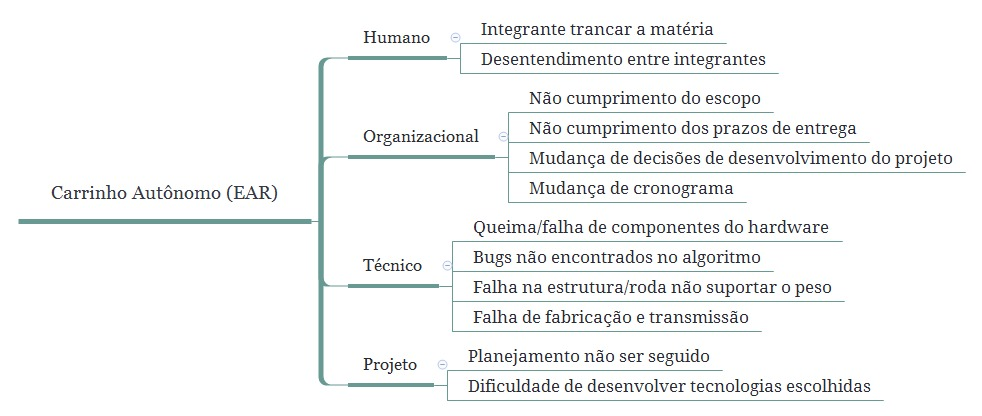
\includegraphics[width=.9\textwidth]{figuras/ear.jpg}
		\caption{Estrutura analítica de Riscos}
		\label{fig:ear}
	\end{figure}

%tabela
% ######## init table ########
\begin{table}[h]
 \centering
% distancia entre a linha e o texto
 {\renewcommand\arraystretch{1.25}
 \caption{Identificação de riscos} \label{tab:identificacao_riscos}
 \begin{tabular}{ l l l l l }
  \cline{1-1}\cline{2-2}\cline{3-3}\cline{4-4}\cline{5-5}  
    \multicolumn{1}{|c|}{\textbf{Erro} \centering } &
    \multicolumn{1}{p{2.550cm}|}{\textbf{Tipo de erro} \centering } &
    \multicolumn{1}{p{1.483cm}|}{\textbf{Impacto} \centering } &
    \multicolumn{1}{p{2.600cm}|}{\textbf{Probabilidade} \centering } &
    \multicolumn{1}{p{1.000cm}|}{\textbf{Risco Rea}l \centering }
  \\  
  \cline{1-1}\cline{2-2}\cline{3-3}\cline{4-4}\cline{5-5}  
    \multicolumn{1}{|p{3.850cm}|}{Integrante trancar a matéria \centering } &
    \multicolumn{1}{p{2.550cm}|}{Humano \centering } &
    \multicolumn{1}{p{1.483cm}|}{2 \centering } &
    \multicolumn{1}{p{2.600cm}|}{1 \centering } &
    \multicolumn{1}{p{1.000cm}|}{4 \centering }
  \\  
  \cline{1-1}\cline{2-2}\cline{3-3}\cline{4-4}\cline{5-5}  
    \multicolumn{1}{|p{3.850cm}|}{Desentendimento entre integrantes \centering } &
    \multicolumn{1}{p{2.550cm}|}{Humano \centering } &
    \multicolumn{1}{p{1.483cm}|}{2 \centering } &
    \multicolumn{1}{p{2.600cm}|}{1 \centering } &
    \multicolumn{1}{p{1.000cm}|}{6 \centering }
  \\  
  \cline{1-1}\cline{2-2}\cline{3-3}\cline{4-4}\cline{5-5}  
    \multicolumn{1}{|p{3.850cm}|}{Não cumprimento do escopo \centering } &
    \multicolumn{1}{p{2.550cm}|}{Organizacional \centering } &
    \multicolumn{1}{p{1.483cm}|}{3 \centering } &
    \multicolumn{1}{p{2.600cm}|}{2 \centering } &
    \multicolumn{1}{p{1.000cm}|}{6 \centering }
  \\  
  \cline{1-1}\cline{2-2}\cline{3-3}\cline{4-4}\cline{5-5}  
    \multicolumn{1}{|p{3.850cm}|}{Não cumprimento dos prazos de entrega \centering } &
    \multicolumn{1}{p{2.550cm}|}{Organizacional \centering } &
    \multicolumn{1}{p{1.483cm}|}{3 \centering } &
    \multicolumn{1}{p{2.600cm}|}{1 \centering } &
    \multicolumn{1}{p{1.000cm}|}{5 \centering }
  \\  
  \cline{1-1}\cline{2-2}\cline{3-3}\cline{4-4}\cline{5-5}  
    \multicolumn{1}{|p{3.850cm}|}{Mudança de decisões de desenvolvimento do projeto \centering } &
    \multicolumn{1}{p{2.550cm}|}{Organizacional \centering } &
    \multicolumn{1}{p{1.483cm}|}{3 \centering } &
    \multicolumn{1}{p{2.600cm}|}{2 \centering } &
    \multicolumn{1}{p{1.000cm}|}{6 \centering }
  \\  
  \cline{1-1}\cline{2-2}\cline{3-3}\cline{4-4}\cline{5-5}  
    \multicolumn{1}{|p{3.850cm}|}{Mudança de cronograma \centering } &
    \multicolumn{1}{p{2.550cm}|}{Organizacional \centering } &
    \multicolumn{1}{p{1.483cm}|}{2 \centering } &
    \multicolumn{1}{p{2.600cm}|}{2 \centering } &
    \multicolumn{1}{p{1.000cm}|}{5 \centering }
  \\  
  \cline{1-1}\cline{2-2}\cline{3-3}\cline{4-4}\cline{5-5}  
    \multicolumn{1}{|p{3.850cm}|}{Queima/falha de componentes do hardware \centering } &
    \multicolumn{1}{p{2.550cm}|}{Técnico \centering } &
    \multicolumn{1}{p{1.483cm}|}{3 \centering } &
    \multicolumn{1}{p{2.600cm}|}{2 \centering } &
    \multicolumn{1}{p{1.000cm}|}{6 \centering }
  \\  
  \cline{1-1}\cline{2-2}\cline{3-3}\cline{4-4}\cline{5-5}  
    \multicolumn{1}{|p{3.850cm}|}{Bugs não encontrados no algoritmo \centering } &
    \multicolumn{1}{p{2.550cm}|}{Técnico \centering } &
    \multicolumn{1}{p{1.483cm}|}{3 \centering } &
    \multicolumn{1}{p{2.600cm}|}{2 \centering } &
    \multicolumn{1}{p{1.000cm}|}{6 \centering }
  \\  
  \cline{1-1}\cline{2-2}\cline{3-3}\cline{4-4}\cline{5-5}  
    \multicolumn{1}{|p{3.850cm}|}{Falha na estrutura/roda não suportar o peso \centering } &
    \multicolumn{1}{p{2.550cm}|}{Técnico \centering } &
    \multicolumn{1}{p{1.483cm}|}{3 \centering } &
    \multicolumn{1}{p{2.600cm}|}{1 \centering } &
    \multicolumn{1}{p{1.000cm}|}{7 \centering }
  \\  
  \cline{1-1}\cline{2-2}\cline{3-3}\cline{4-4}\cline{5-5}  
    \multicolumn{1}{|p{3.850cm}|}{Falha de fabricação e transmissão \centering } &
    \multicolumn{1}{p{2.550cm}|}{Técnico \centering } &
    \multicolumn{1}{p{1.483cm}|}{3 \centering } &
    \multicolumn{1}{p{2.600cm}|}{2 \centering } &
    \multicolumn{1}{p{1.000cm}|}{7 \centering }
  \\  
  \cline{1-1}\cline{2-2}\cline{3-3}\cline{4-4}\cline{5-5}  
    \multicolumn{1}{|p{3.850cm}|}{Dificuldade de desenvolver tecnologias escolhidas \centering } &
    \multicolumn{1}{p{2.550cm}|}{Projeto \centering } &
    \multicolumn{1}{p{1.483cm}|}{2 \centering } &
    \multicolumn{1}{p{2.600cm}|}{2 \centering } &
    \multicolumn{1}{p{1.000cm}|}{5 \centering }
  \\  
  \cline{1-1}\cline{2-2}\cline{3-3}\cline{4-4}\cline{5-5}  
    \multicolumn{1}{|p{3.850cm}|}{Planejamento não ser seguido \centering } &
    \multicolumn{1}{p{2.550cm}|}{Projeto \centering } &
    \multicolumn{1}{p{1.483cm}|}{2 \centering } &
    \multicolumn{1}{p{2.600cm}|}{1 \centering } &
    \multicolumn{1}{p{1.000cm}|}{4 \centering }
  \\  
  \hline

 \end{tabular} }
\end{table}

\newpage

\subsection{Definição de respostas a riscos}
Uma vez que os riscos foram identificados, devem-se ser consideradas medidas de tratamento desses erros, considerando os recursos dispostos e a viabilidade dessas soluções.
\par Para isso, são caracterizadas possíveis medidas de correção do erro.

\textbf{Evitar:} 
Modificando o plano de projeto para eliminar a possibilidade, mesmo que não completamente, mas podendo ser evitado.

\textbf{Transferir:} 
Fazer com que sua consequência se torne parte de uma resposta, transferindo-a para outra parte.

\textbf{Mitigar:} 
Reduzir sua consequência, de forma a propor ações preventivas para que sejam mínimas.
 
\par Dessa forma, estratégias são aplicadas aos erros conforme a define a Tabela \ref{tab:estrategia_riscos}.

%tabela
% ######## init table ########
\begin{table}[h]
 \centering
% distancia entre a linha e o texto
 {\renewcommand\arraystretch{1.25}
 \caption{Estratégia para riscos} \label{tab:estrategia_riscos}
 \begin{tabular}{ l l }
  \cline{1-1}\cline{2-2}  
    \multicolumn{1}{|c|}{\textbf{Erro} \centering } &
    \multicolumn{1}{c|}{\textbf{Correção} \centering }
  \\  
  \cline{1-1}\cline{2-2}  
    \multicolumn{1}{|p{3.850cm}|}{Integrante trancar a matéria \centering } &
    \multicolumn{1}{p{4.217cm}|}{Transferir \centering }
  \\  
  \cline{1-1}\cline{2-2}  
    \multicolumn{1}{|p{3.850cm}|}{Desentendimento entre integrantes \centering } &
    \multicolumn{1}{p{4.217cm}|}{Mitigar \centering }
  \\  
  \cline{1-1}\cline{2-2}  
    \multicolumn{1}{|p{3.850cm}|}{Não cumprimento do escopo \centering } &
    \multicolumn{1}{p{4.217cm}|}{Evitar \centering }
  \\  
  \cline{1-1}\cline{2-2}  
    \multicolumn{1}{|p{3.850cm}|}{Não cumprimento dos prazos de entrega \centering } &
    \multicolumn{1}{p{4.217cm}|}{Evitar \centering }
  \\  
  \cline{1-1}\cline{2-2}  
    \multicolumn{1}{|p{3.850cm}|}{Mudança de decisões de desenvolvimento do projeto \centering } &
    \multicolumn{1}{p{4.217cm}|}{Evitar \centering }
  \\  
  \cline{1-1}\cline{2-2}  
    \multicolumn{1}{|p{3.850cm}|}{Mudança de cronograma \centering } &
    \multicolumn{1}{p{4.217cm}|}{Mitigar \centering }
  \\  
  \cline{1-1}\cline{2-2}  
    \multicolumn{1}{|p{3.850cm}|}{Queima/falha de componentes do hardware \centering } &
    \multicolumn{1}{p{4.217cm}|}{Mitigar \centering }
  \\  
  \cline{1-1}\cline{2-2}  
    \multicolumn{1}{|p{3.850cm}|}{Bugs não encontrados no algoritmo \centering } &
    \multicolumn{1}{p{4.217cm}|}{Mitigar \centering }
  \\  
  \cline{1-1}\cline{2-2}  
    \multicolumn{1}{|p{3.850cm}|}{Falha na estrutura/roda não suportar o peso \centering } &
    \multicolumn{1}{p{4.217cm}|}{Mitigar \centering }
  \\  
  \cline{1-1}\cline{2-2}  
    \multicolumn{1}{|p{3.850cm}|}{Falha de fabricação e transmissão \centering } &
    \multicolumn{1}{p{4.217cm}|}{Mitigar \centering }
  \\  
  \cline{1-1}\cline{2-2}  
    \multicolumn{1}{|p{3.850cm}|}{Dificuldade de desenvolver tecnologias escolhidas \centering } &
    \multicolumn{1}{p{4.217cm}|}{Mitigar \centering }
  \\  
  \cline{1-1}\cline{2-2}  
    \multicolumn{1}{|p{3.850cm}|}{Planejamento não ser seguido \centering } &
    \multicolumn{1}{p{4.217cm}|}{Evitar \centering }
  \\  
  \hline

 \end{tabular} }
\end{table}























\chapter{Biblioteca de funções para o processamento de imagens}

\lstinputlisting[language=Python]{codigos/library.py}

\end{apendicesenv}
